\documentclass[a4paper]{article}

\usepackage{tikz}
\usepackage{a4wide}
\usepackage{amsmath}
\usepackage{hyperref}
\usepackage{cleveref}

\usetikzlibrary{calc,intersections}

\newcommand{\coords}[3]{\ensuremath{(#1,#2,#3)}}

\begin{document}

\section{Math}

\begin{center}
    \begin{tabular}{cc}
        \begin{tikzpicture}[measure/.style={ultra thin,<->},
                            measure label/.style={midway,above,sloped,font=\tiny,inner sep=1pt},
                            guide/.style={ultra thin,dashed},
                            eye ray/.style={red},
                            axis/.style={-latex,blue,thin},
                            axis label/.style={blue}]
            \coordinate (eye) at (0,-1);
            \coordinate (object) at (-1,1.5);
            \coordinate (viewplane left) at (-2,0);
            \coordinate (viewplane right) at (2,0);

            \path[use as bounding box] (-2.5,-2) rectangle (2.5,2.5);

            \draw[axis] (-1,0) -- (2.5,0) node[axis label,above] {X};
            \draw[axis] (0,-1) -- (0,2.5) node[axis label,right] {Z};

            \draw[fill] (eye) circle[radius=1pt] node[below,font=\tiny] {E};
            \draw[fill] (object) circle[radius=1pt] node[above,font=\tiny] {P};
            \draw[thick,name path=view plane] (viewplane left) -- (viewplane right);
            \draw[eye ray,name path=eye ray] (eye) -- (object);
            \path[name intersections={of=view plane and eye ray, by=projection}];
            \draw[fill,red] (projection) circle[radius=1pt] node[above right,font=\tiny,inner sep=1pt] {P'};

            \draw[guide] let \p1=(eye) in (\p1) -- (-2.5,\y1);
            \draw[guide] let \p1=(viewplane left) in (\p1) -- (-2.5,\y1);
            \draw[guide] let \p1=(object) in (\p1) -- (-2.5,\y1);
            \draw[guide] let \p1=(object) in (\p1) -- (\x1,2);
            \draw[guide] let \p1=(projection) in (\p1) -- (\x1,1.75);
            \draw[measure] let \p1=(eye), \p2=(projection) in (-2.5,\y1) -- (-2.5,\y2) node[measure label] {$d$};
            \draw[measure] let \p1=(projection), \p2=(object) in (-2.5,\y1) -- (-2.5,\y2) node[measure label] {$z$};
            \draw[measure] let \p1=(eye), \p2=(object) in (\x1,2) -- (\x2,2) node[measure label] {$x$};
            \draw[measure] let \p1=(eye), \p2=(projection) in (\x1,1.75) -- (\x2,1.75) node[measure label] {$x'$};
        \end{tikzpicture}
        &
        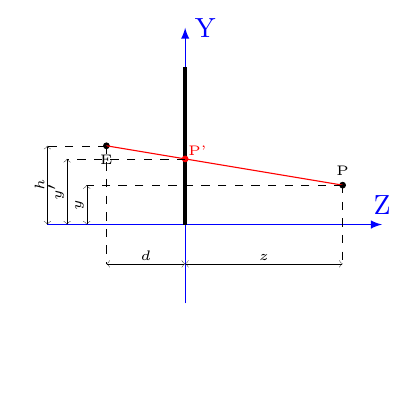
\begin{tikzpicture}[measure/.style={ultra thin,<->},
                            measure label/.style={midway,above,sloped,font=\tiny,inner sep=1pt},
                            guide/.style={ultra thin,dashed},
                            eye ray/.style={red},
                            axis/.style={-latex,blue,thin},
                            axis label/.style={blue}]
            \coordinate (eye) at (-1,1);
            \coordinate (object) at (2,0.5);
            \coordinate (viewplane top) at (0,0);
            \coordinate (viewplane bottom) at (0,2);

            \path[use as bounding box] (-2,-2) rectangle (2.5,2.5);

            \draw[axis] (-1.75,0) -- (2.5,0) node[axis label,above] {Z};
            \draw[axis] (0,-1) -- (0,2.5) node[axis label,right] {Y};

            \draw[fill] (eye) circle[radius=1pt] node[below,font=\tiny] {E};
            \draw[fill] (object) circle[radius=1pt] node[above,font=\tiny] {P};
            \draw[ultra thick,name path=view plane] (viewplane bottom) -- (viewplane top);
            \draw[eye ray,name path=eye ray] (eye) -- (object);
            \path[name intersections={of=view plane and eye ray, by=projection}];
            \draw[fill,red] (projection) circle[radius=1pt] node[above right,font=\tiny,inner sep=1pt] {P'};

            \draw[guide] let \p1=(eye) in (\p1) -- (-1.75,\y1);
            \draw[guide] let \p1=(projection) in (\p1) -- (-1.5,\y1);
            \draw[guide] let \p1=(object) in (\p1) -- (-1.25,\y1);
            \draw[guide] let \p1=(eye) in (\p1) -- (\x1,-0.5);
            \draw[guide] let \p1=(object) in (\p1) -- (\x1,-0.5);
            \draw[measure] let \p1=(eye) in (-1.75,0) -- (-1.75,\y1) node[measure label] {$h$};
            \draw[measure] let \p1=(projection) in (-1.5,0) -- (-1.5,\y1) node[measure label] {$y'$};
            \draw[measure] let \p1=(object) in (-1.25,0) -- (-1.25,\y1) node[measure label] {$y$};
            \draw[measure] let \p1=(eye) in (\x1,-0.5) -- (0,-0.5) node[measure label] {$d$};
            \draw[measure] let \p1=(object) in (\x1,-0.5) -- (0,-0.5) node[measure label] {$z$};
        \end{tikzpicture} \\
        \textbf{From Above} & \textbf{From Side} \\
    \end{tabular}
\end{center}

Basic setup:
\begin{itemize}
    \item View plane represents screen
          \begin{itemize}
            \item Coincides with XY plane
            \item Is the plane upon which we need to project objects
          \end{itemize}
    \item Eye represents camera
          \begin{itemize}
            \item At a distance $d$ from view plane ($d$ can be chosen freely, suggested value: $1$)
            \item At a height $h$ from the ground
            \item Therefore has coordinates $\coords{0}{h}{-d}$
          \end{itemize}
    \item Point $P$
          \begin{itemize}
            \item Represents location in 3D world
            \item Has coordinates $\coords{x}{y}{z}$
          \end{itemize}
    \item Point $P'$
          \begin{itemize}
            \item Represents projection of $P$ on view plane
            \item Has coordinates $\coords{x'}{y'}{0}$
          \end{itemize}
\end{itemize}

\subsection{General Algorithm}

We are given
\begin{itemize}
    \item Two points $P$ and $Q$.
    \item A plane going through some point $O$ and normal vector $\vec{N}$.
\end{itemize}

Goal: draw a ray $R(t)$ through $P$ and $Q$ and find intersection with plane.

In practice, we will take the eye as $P$, the game object as $Q$ and the view plane as intersection plane (but also other combinations, see below).

\begin{align*}
    R(t) & = P + (Q - P) \cdot t \\
    t & = \frac{(O-P) \cdot N}{(Q-P) \cdot N} \\
    P' & = R(t) \\
       & = P + (Q - P) \cdot \frac{(O-P) \cdot N}{(Q-P) \cdot N} \\
\end{align*}

\subsection{World to View Plane}\label{sec:world2view}

We choose appropriate values for $P$, $Q$, $O$ and $\vec{N}$:

\begin{align*}
    O & = \coords{0}{0}{0} \\
    P & = \coords{0}{h}{-d} \\
    Q & = \coords{x}{y}{z} \\
    \vec{N} & = \coords{0}{0}{1} \\
\end{align*}

This gives

\begin{align*}
    t & = \frac{d}{z + d} \\ \\
    P' & = \coords{x \cdot t}{h + (y - h) \cdot t}{0}
\end{align*}

\subsection{View Plane to World} \label{sec:view2world}

Conversely, we can start off on a point $P'$ on the view plane and determine which world point $P$ would be projected on this $P'$.
The problem is that there is an infinitude of such points: all points on the ray through the eye $E$ and $P'$ get projected onto $P'$.
This means we need an extra constraints.

We intend to use this reverse algorithm to determine where to draw the road, so finding a $P$ whose $z$-coordinate is $0$ could come in handy.

\begin{align*}
    O & = \coords{0}{0}{0} \\
    P & = \coords{x}{y}{0} \\
    E & = \coords{0}{h}{-d} \\
    N & = \coords{0}{1}{0} \\
\end{align*}

This leads to

\begin{align*}
    t & = \frac{h}{h-y} \\
    P' & = \coords{x \cdot t}{0}{(t - 1) \cdot d}
\end{align*}

\subsection{View Plane to Screen}\label{sec:view2screen}

Say our screen coincides with the square $[-0.5,0.5] \times [0,1]$ in the view plane. (Technically this should be a rectangle with the same aspect ratio as the screen, but too lazy.)
We need to translate these coordinates into screen coordinates $P''(x'', y'', z'')$ in the rectangle $[0,W] \times [0,H]$ (e.g., with $W=640$ and $H=480$).

\begin{align*}
    x'' = \left\lfloor x' \cdot W + \frac{W}{2} \right\rfloor \\
    y'' = \left\lfloor (1-y') \cdot H \right\rfloor \\
\end{align*}

\subsection{Screen to View Plane}\label{sec:screen2view}

Inverse operation.

\begin{align*}
    x' = \frac{(x'' - \frac{W}{2})}{W} \\
    y' = 1 - \frac{y''}{H} \\
\end{align*}


\section{Algorithms}

\subsection{Drawing the Road}

Normally you would choose a point on the road and project it onto the view plane. However, the road is infinitely long and
far away road segments would be projected onto the same row of pixels.

To avoid that, we turn things around:
\begin{itemize}
    \item Say we want to determine how to draw the road on the screen row with coordinate $y''$.
    \item We look for the corresponding $P' \coords{0}{y'}{0}$ point on the view plane (\cref{sec:screen2view}).
    \item We shoot a ray through $E$ and $P'$.
    \item We look where this ray hits the ground: $P(0,0,z)$ (\cref{sec:view2world}). $z$ tells us how far away the road segment that we need to draw is.
    \item We pick take the point $P_2(w/2,0,z)$ that falls on the edge of the road. $w$ stands for the width of the road.
    \item We project $P_2$ back on the view plane (\cref{sec:world2view}), which yields $P_2'(x'_2, y'_2, 0)$. $x'_2$ indicates how wide the row should be drawn on the screen:
          the road's projection spans from $-x'_2$ to $x'_2$ in the view plane.
    \item Convert the view plane coordinates to screen coordinates (\cref{sec:view2screen}).
\end{itemize}

\subsection{Drawing an Object}

\begin{itemize}
    \item Say the object is located at $P(x, y, z)$.
    \item Project $P$ onto the view plane (\cref{sec:world2view}). This gives $P'(x', y', 0)$.
    \item Convert these coordinates to screen coordinates (\cref{sec:view2screen}).
\end{itemize}

You might need to know the \emph{size} of the projection. This can be achieved by seeing the objects as a rectangle.
Take two opposing corners, call them $P$ and $Q$. Project them both onto the view plane, yielding $P'$ and $Q'$.
Taking the difference of their coordinates yields the width and height of the projected object.

\end{document}